\section{Grafsk bruger interface}
\textit{Dette afsnit omhandler design, implementering og test af GUI, til visualisering af de udførte aktiviteter. Først designes GUI til det specifikke formål udfra dets kravspecifikationer, hvorefter denne kan implementeres. Afslutningsvist bliver GUI testet i forhold til opstillede krav.}
\subsection{Design}
GUI benyttes til at motivere børn til en mere aktiv hverdag. Dette gøres ud fra \secref{motivation_boern}, hvor det beskrives at børn motiveres gennem succesoplevelser. GUI designes dermed ud fra at alle børn har mulighed for at optjene mange point, da pointene vægtes ud fra intensiteten, tiden samt typen af aktivitet.

Data fra algoritmerne vedrørende aktiviteterne gang, løb og cykling sendes til MATLAB, som det ses på \figref{fig:GUI}. Fra algoritmen vedrørende gang og løb sendes der to resultater. Resultaterne består i en peakværdi og et resultat af varighed siden sidst detekterede peak. Peakets værdi informere om hvilken aktivitet på baggrund af dets størrelse, varigheden bør tillægges. Fra algoritmen vedrørende cykling sendes der et resultat til MATLAB bestående af varigheden for udført cykling. Fra algoritmen vedrørende pulssensoren sendes data i form af BPM, beregnet over tre peaks. \\
Der er fastsat en tærskelværdi for gang, løb og cykling, hvoraf GUI modtager resultater fra algoritmerne. Ved gang, løb og cykling modtages varigheden som samples og skal dermed omregnes til tid. For at omregne dette til en faktor bestående af tid, skal det modtagne resultat divideres med samplingsfrekvensen. Herefter ligges tiden over i en tidsvariabel for den tilhørende aktivitet. Denne vises som værdi for den enkelte aktivitet, så det er muligt at se hvor længe barnet har været aktiv ved de forskellige aktiviteter.

Hver aktivitet belønnes forskelligt, da det er væsentligt at få børnene til at løbe og cykle mere, end blot at gå. Dermed ganges tiden for løb med tre, for cykling med to og for gang med en. Derudover belønnes barnet for intensiteten af aktiviteten. Aktivitetens point ganges med to ved høj intensitet, ganges med halvanden ved moderat intensitet, og ganges ikke ved lav intensitet. Pointene visualiseres ud for den enkelte aktivitet, så barnet kan se hvor mange point de har opnået ved udførslen for den enkelte aktivitet igennem en hel dag. For at aktivere børnene hver dag, samles dagens point for alle aktiviteter udført i løbet af dagen. Pointene vises grafisk som en søjle hvormed barnet nemt kan få et overblik over antallet af point fra de forskellige dage. Søjlen afspejler hvor mange point børnene har opnået samt hvor stor en del der er opnået ved henholdsvis gang, løb og cykling.  

\begin{figure}[H]
	\centering
	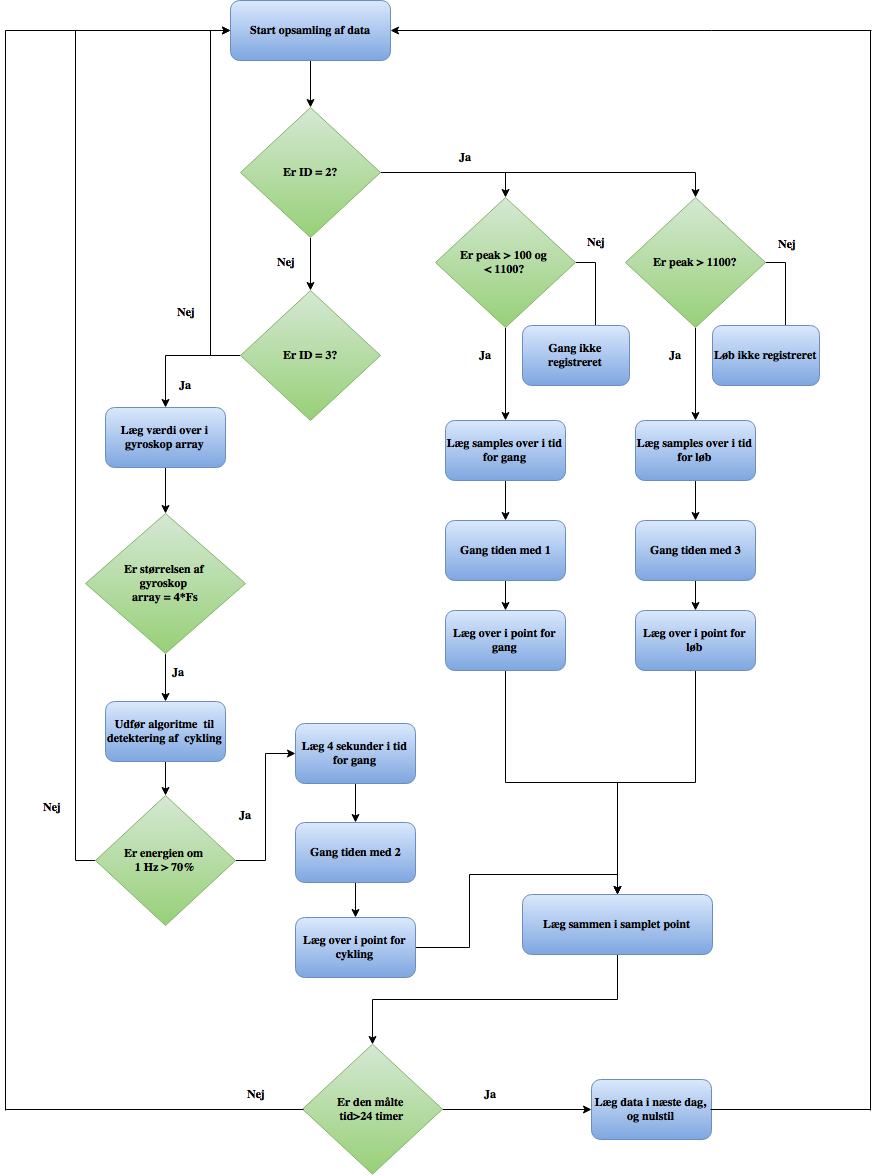
\includegraphics[scale=0.4]{figures/cDesign/pseudo_GUI.png}
	\caption{På figuren ses et flowchart som gennemgår hvorledes resultaterne fra de forskellige algoritmer behandles af GUI.}
	\label{fig:GUI}
\end{figure}

\subsection{Implementering}
GUI implementeres ved at anvende MATLABS funktion Graphical User Interface Design Environment (GUIDE). GUIDE er en funktion der gør det muligt at lave en specifik brugerflade med indbyggede funktioner. I GUIen benyttes en toggle button for at starte og slutte indsamling af resultater fra algoritmerne vedrørende aktiviteterne gang, løb og cykling. Derudover benyttes axes, som benyttes til at repræsentere de samlede point der er samlet i løbet af dagen. Sidst benyttes static text til de resterende funktioner i GUI. \newline
Resultaterne fra algoritmen vedrørende gang og løb sendes til MATLAB, hvor de gemmes i en variabel med [samples, peak]. Resultaterne fra algoritmen vedrørende cykling sendes til MATLAB, og gemmes i en variable med [samples, C]. Begge algoritmers resultater sammenholdes med resultaterne fra algoritmen vedrørende pulsdetektering med henblik på multiplikation afhængig af intensitetsniveau. Resultatet fra pulsdetektering sendes til MATLAB og gemmes i en variable med [BPM].

\subsubsection{Test}
GUIs funktionalitet testes ud fra kravene heraf, se \secref{krav_GUI}. Dets funktionalitet testes ved at indsende kendte værdier, hvoraf hver aktivitet kan testes individuelt. Igennem en test med kendte værdier kan funktionen med multiplikation af point afhængig af aktivitetstype, varighed, multiplikation af point vedrørende intensitet og aktivitetstype genkendelse, testes igennem samme test.
Igennem testen indsendes følgende datasæt som skulle trigge de forskellige aktiviteter. Dataene skal fungere som simulerede input fra algoritmerne. 
\begin{eqnarray*}
	Gang &=& [512~110,~512~110,~512~110,~512~110,~512~110,~512~110] \\ 
	L\text{ø}b &=& [512~1110,~512~1110,~512~1110,~512~1110,~512~1110] \\ 
	Cykling &=& [512~C,~512~C,~512~C,~512~C,~512~C,~512~C] \\
	Lav\text{ }intensitet &=& [146~146~146~146~146~146] \\ 
	Middel\text{ }intensitet &=& [147~147~147~147~147~147] \\ 
	H\text{ø}j\text{ }intensitet &=& [168~168~168~168~168~168] 
\end{eqnarray*}
Resultatet af GUIs design så skal forskellige aktivitetsformer bidrage til en forskellig mængde point. Ligeledes er varigheden og intensiteten  af aktiviteten afgørende for mængden af opnåede point, på baggrund af deres multiplikationsfaktor. Testen udføres med ovenstående data, en test for hvert intensitetsniveau. Måden hvorpå pointene udregnes, og dermed varierer, afhænger af aktiviteten samt intensiteten, hvilket ses i nedenstående ligning. 
\begin{equation*}
Antal point = \frac{Samples}{Samplingsfrekvens} \cdot Aktivitetsfaktor \cdot Intensitetsfaktor
\end{equation*}
Varigheden udregnes som nævnt i design ved at dividere modtagne antal samples med samplingsfrekvensen. Resultatet heraf betyder at for alle test indsendes der 6 sekunder af hver aktivitet, hvis samplingsfrekvensen var 512, som i pilotforsøget.
\begin{table}[H]
	\centering
	\begin{tabular}{cccc}
		\hline
		\rowcolor[HTML]{C0C0C0} 
		Aktivitet & Indsendt data & Forventet antal point & Optalt antal point \\ \hline
		Gang & Gang - Lav intensitet & 6 & 6 \\ \hline
		Gang & Gang - Middel intensitet & 9 & 9 \\ \hline
		Gang & Gang - Høj intensitet & 12 & 12 \\ \hline
		Løb & Løb - Lav intensitet & 18 & 18 \\ \hline
		Løb & Løb - Middel intensitet & 27 & 27 \\ \hline
		Løb & Løb - Høj intensitet & 36 & 36 \\ \hline
		Cykling & Cykling - Lav intensitet & 12 & 12 \\ \hline
		Cykling & Cykling - Middel intensitet & 18 & 18 \\ \hline
		Cykling & Cykling - Høj intensitet & 24 & 24 \\ \hline
	\end{tabular}
	\caption{I tabellen ses sammenhængen mellem forventede antal point og optalt antal point, som resultat af den indsendte simulerede data.}
	\label{test:GUI}
\end{table}\vspace{-.5cm}
På baggrund af testen af GUI, kunne det konkluderes at denne fungerer efter hensigten. De forventede antal point og optalt antal point var nøjagtig det samme. Disse optjente point visualiseres i et søjlediagram som beskrevet i design. Varigheden af hvert aktivitet visualiseres som en boks, som summeres op hver gang et aktivitetsresultat bliver behandlet. Resultatet af at indsende det simulerede data afspejles i GUI i nedenstående figur.

\textit{\textbf{Figur indsættes her, include er udkommenteret.} }
%\begin{figure}[H]
%	\centering
%	\includegraphics[scale=0.4]{figures/cDesign/test_gui_matlab.png}
%	\caption{På figuren ses et udklip af GUI hvor udførslen af aktiviteterne gang, løb og cykling visualiseres. Aktiviteternes samlede antal point og udført varighed ses på figuren.}
%	\label{fig:GUI}
%\end{figure}

Efterfulgt af design, implementering og test af GUI, kan det konkluderes at denne opfylder kravene heraf. GUI er i stand til at visualisere tidsforbruget samt antal point opnået, for alle aktiviteterne. GUI opdaterede i testen i reelle tid, hvoraf kravet vedrørende opdatering af GUI mindst hvert femtende minut, ligeledes er opfyldt.